	\documentclass[letterpaper, 10 pt, conference]{ieeeconf}  % Comment this line out if you need a4paper

%\documentclass[a4paper, 10pt, conference]{ieeeconf}      % Use this line for a4 paper

\IEEEoverridecommandlockouts                              \overrideIEEEmargins       

% See the \addtolength command later in the file to balance the column lengths
% on the last page of the document

% The following packages can be found on http:\\www.ctan.org
\usepackage{graphics} % for pdf, bitmapped graphics files
\usepackage{epsfig} % for postscript graphics files
\usepackage{mathptmx} % assumes new font selection scheme installed
\usepackage{times} % assumes new font selection scheme installed
\usepackage{amsmath} % assumes amsmath package installed
\usepackage{amssymb}  % assumes amsmath package installed
\usepackage{algpseudocode}
\usepackage[dvipsnames]{xcolor}% http://ctan.org/pkg/xcolor
\usepackage{algorithm}
\usepackage{comment}
\usepackage{tabularx}
\usepackage{capt-of}
\usepackage{lipsum} %used to generate dummy text
\usepackage{calc}
\usepackage{bbm}
\usepackage{mathtools}

\makeatletter
\newcommand{\algcolor}[2]{%
  \hskip-\ALG@thistlm\hspace*{-\fboxsep}\colorbox{#1}{\parbox{\dimexpr\linewidth-2\fboxsep}{\hskip\ALG@thistlm\relax #2}}%
}
\newcommand{\algemph}[1]{\algcolor{lightgray}{#1}}
\makeatother

%\usepackage{caption}

\DeclareMathOperator*{\argmin}{arg\,min}
\DeclareMathOperator{\argminG}{arg\,min}  
\DeclareMathOperator*{\argmax}{arg\,max}
\DeclareMathOperator{\argmaxG}{arg\,max}
\newcommand\bigforall{\mbox{\Large $\mathsurround0pt\forall$}} 
\newcommand{\pluseq}{\mathrel{+}=}
\newcommand{\norm}[1]{\left\lVert#1\right\rVert_1}
\def\HiLi{\leavevmode\rlap{\hbox to \hsize{\color{yellow!50}\leaders\hrule height .8\baselineskip depth .5ex\hfill}}}

\title{\LARGE \bf Combining artificial curiosity and tutor guidance in a virtual agent for environment exploration}


\author{Pierre Fournier$^{1}$, Olivier Sigaud$^{1}$ and Mohamed Chetouani$^{1}$% <-this % stops a space
\thanks{*This work was not supported by any organization}% <-this % stops a space
\thanks{$^{1}$ The authors are with: Sorbonne Universit\'es, UPMC Univ Paris 06, CNRS UMR 7222, Institut des Syst\`emes Intelligents et de Robotique, F-75005 Paris, France Contact: {\tt pierre.fournier@isir.upmc.fr} +33 (0) 1 44 27 88 53}%
}


\begin{document}



\maketitle
\thispagestyle{empty}
\pagestyle{empty}

%%%%%%%%%%%%%%%%%%%%%%%%%%%%%%%%%%%%%%%%%%%%%%%%%%%%%%%%%%%%%%%%%%%%%%%%%%%%%%%%
\begin{abstract}
In a new environment, an artificial agent should explore autonomously and exploit tutoring signals from human caregivers. While these two mechanisms have mainly been studied separately, we show in this paper that a carefully designed combination of both performs better than each separately. To this end, we propose an autonomous agent whose actions result from a user-defined weighted combination of two drives: a tendency for gaze-following behaviors in presence of a tutor, and a novelty-based intrinsic curiosity, both incorporated in a model-based reinforcement learning framework through reward shaping. The agent is evaluated on a discretized pick-and-place task in order to explore the effects of various combinations of both drives. Results show how a properly tuned combination leads to a faster and more consistent discovery of the task over each drive in isolation. Additionally, experiments in a non-rewarding version of the environment indicate that combining curiosity and gaze-following behaviors is a promising path for real-life exploration in artificial agents.

\begin{comment}
In order to learn what to do, artificial agents should perform autonomous exploration of their environment while making profit of tutoring signals from a human caregiver.
In this paper, we propose a model which combines both components through a tendency to follow the gaze of the tutor.
We show that this combination performs better than both mechanisms in isolation after tuning the respective weights of autonomous exploration and gaze following.
\end{comment}

\end{abstract}
%%%%%%%%%%%%%%%%%%%%%%%%%%%%%%%%%%%%%%%%%%%%%%%%%%%%%%%%%%%%%%%%%%%%%%%%%%%%%%%%

\begin{comment}

the use of robots in sectors where they need to interact with humans grows, new requirements and challenges arise, among which lies the capability for them to both act autonomously in real life conditions and at the same time learn from humans around. This study is set in the context where a robot is discovering an unknown environment, and addresses the question: how could a human tutor speed up this discovery and orient it through natural interaction only ? These objectives are related to similar questions in the realm of developmental cognitive sciences and developmental psychology: how do babies and infants acquire knowledge of their surroundings cumulatively, and how do they make the best use of their parents' tutoring in this respect ? Task-independent lifelong learning of increasingly complex skills in artificial embodied systems, with inspiration from human children, has become a well-defined field of research known as developmental robotics. This work comes at the intersection of developmental robotics, reinforcement learning and Human-Robot Interaction and proposes to answer the initial question posed by augmenting the intrinsically motivated reinforcement learning framework with an attentional layer that favors synchrony with an identified tutor, so as to enable a primitive form of information transfer between the two.

\subsection{Intrinsically motivated reinforcement learning}

Before augmenting a robot's capabilities through interaction with a tutor, it must be able to learn autonomously in an unknown environment. The recent successes of the reinforcement learning framework at learning complex tasks from scratch, be it in the robotic field or in pure machine learning, make it a promising candidate to be the natural learning framework of a developing embodied system. But its initial paradigm is flawed in a number of respects to meet developmental constraints: reward engineering often leads to poor task independence, and the concept of a naturally rewarding environment itself is questionable, as primitive reward signals like pain do not drive learning in most cases. These two limitations have been partially overcome by the introduction of intrinsic motivation, which states that the drive to learn new competences, engage exploration of a new environment or simply play originates from an internal mechanism that can do without any explicitly rewarding external signal. Rather than being optimized for a given task, an intrinsically motivated system is encouraged to acquire undirected, high level and generalizable capabilities that can become building-blocks to more directed behavior when needed. This approach is more suitable to develop naturally curious behaviors, as requires the environment discovery setup, and this work adopts it.

\subsection{Interactive learning through attention coordination}

By leveraging progresses made in human-robot interaction, 

\subsection{Intrinsic motivation and model-based reinforcement learning}




Intrinsically motivated reinforcement learning: this works focus on building a collection of reusable skills through the semi-Markov decision processes framework. Learning option models make it possible to transfer learning from task to task through these options. The intrinsic motivation originates in a notion of saliency and is described as the mechanism at play to define new options. Unfortunately the salient nature of events is predefined and does not emerge from broader considerations in this work, which reduces its interest in terms of autonomy and adaptability.

 



Intrinsic VS extrinsic / external VS internal: What is intrinsic motivation? A typology of computational approaches

Playroom experiment, metamodel to evaluate performance on model, Intelligent Adaptive Curiosity, not based on reinforcement learning, sensorimotor models, Intrinsic Motivation Systems for Autonomous
Mental Development

Active learning approach, Active Learning for Autonomous Intelligent Agents:
Exploration, Curiosity, and Interaction

Model-based reinforcement learning, montecarlo based simulation, UCT algorithm 

Hester Stone texplore

Emergent structuring of interdependent affordance learning tasks

From human instructions to robot actions: Formulation of goals, affordances and probabilistic planning
 
Improving reinforcement learning with interactive feedback and affordances
Learning object affordances by leveraging the combination of human-guidance and self-exploration

Travaux d'anis: unsupervised guidance
From Motor Learning to Interaction Learning in Robots, Olivier

Learning behavior for a social interaction game with a childlike humanoid robot

explauto, goal babbling,
Active learning of inverse models with intrinsically motivated goal exploration in robots
Intrinsic motivation systems for autonomous mental development
\end{comment}

\section{Introduction}

Mental development for a situated agent includes the capacity to actively discover how to achieve various tasks in an unknown environment. Young children demonstrate very early the inclination to explore their surroundings, trying to interact with objects within their reach. In artificial systems, these behaviors are the subject of Artificial Curiosity. Taking inspiration from trial-and-error exploration, some of the existing work is built on the Reinforcement Learning (RL) framework \cite{sutton_reinforcement_1998}. Such solutions, called intrinsically motivated reinforcement learning (IMRL) \cite{oudeyer_what_2009}, rely on attractive salient events \cite{chentanez_intrinsically_2004} or search to maximize metrics of their environment model \cite{hester_intrinsically_2012}. A limitation of the RL framework for autonomous environment exploration is the notion of external reward. Indeed, such rewards are most commonly human-engineered task-specific functions \cite{dewey_reinforcement_2014} that cannot be defined in the essentially task-independent exploration problem, nor redefined for every new environment. 

When in presence of a caregiver, infants are also able to incorporate social stimuli into their exploration behavior (following a tutor gaze, copying gestures, ...), long before the acquisition of an effective language-like high-level communication channel. In this context, social signals can favor task exploration and guide it towards the expectations of a tutor. Such ability to exploit skills and knowledge from humans in artificial systems is the subject of Interactive Machine Learning (IML) \cite{senft_leveraging_2017}. IML algorithms can be organized along a scale between focusing entirely on human guidance \cite{fern_decision-theoretic_2014} versus relying only on autonomous exploration \cite{griffith_policy_2013}. Between those extremes, the combination between human guidance and autonomous exploration can provide better results, to learn object affordances for example \cite{chu_learning_2016}.

The present work pushes the latter approach further by proposing a generic RL system where motivations to explore and to interact are both externally tunable, and shows that the right proportion of each leads to increased performances on task-discovery and task execution in a new environment. To this end, we propose an agent whose actions respond to a user-defined weighted average of two incentives: artificial curiosity on one side, and a tendency to follow the gaze of a tutor on the other side. 
%Taking inspiration from developmental psychology, the coordination is based on a motivation mechanism that entices the agent to follow its tutor gaze. 

The artificial curiosity component is based on the intrinsically motivated RL algorithm of \textsc{texplore-vanir} \cite{hester_intrinsically_2012}.
The gaze-following component, which is considered essential to learn to interact \cite{nomikou_constructing_2016, kaplan_challenges_2006}, is implemented through the addition of gaze direction in the \textsc{texplore-vanir} agent and the use of a new reward shaping mechanism that entices the agent to match its gaze with the tutor's.

After presenting \textsc{texplore-vanir} in Section~\ref{background}, our method and the simulated task are described in Section~\ref{methods}. Results are presented in Section~\ref{results}. First, we show that with a simple gaze policy for the tutor, the right weights for both curiosity and gaze-following behaviors lead to improved performances for task discovery and execution. Following remarks on external rewards in RL settings, we also show that our agent can consistently complete the task in non-rewarded environments. Finally, Section~\ref{conclusion} discusses the originality of this work in comparison with the existing literature, gives potential directions for future work and concludes.

\section{Background: \textsc{texplore-vanir}}
\label{background}

The \textsc{texplore-vanir} algorithm is an improvement of the \textsc{texplore} model-based reinforcement learning framework \cite{hester_texplore:_2013} that includes additional intrinsic motivations.

\subsection{\textsc{Texplore}}

The \textsc{texplore} algorithm follows a typical model-based RL scheme, where the environment is modeled as a factored Markov Decision Process (MDP). A MDP consists of a set of states $S$, a set of actions $A$, a reward function $R(s,a)$ and a transition function $T(s,a,s')$. The agent receives the reward $R(s,a)$ upon taking action $a$ in state $s$ and ends up in state $s'$ with probability $P(s'|s,a) = T(s,a,s')$. The agent seeks to determine the policy $\pi^\star: s \mapsto a$ that maximizes the expected discounted total reward over the agent lifetime. Defining the state-value function $Q^{\pi}(s,a)$ as an estimate of the expected future reward obtainable from $(s,a)$ following policy $\pi$, $Q^\star = Q^{\pi^\star}$ solves the Bellman equation \cite{sutton_reinforcement_1998} and 
\begin{equation}
\pi^\star(s) = \argmax_{a} Q^{\star}(s,a).
\end{equation} 
Being model-based, the \textsc{texplore} agent learns models of $R$ and $T$ from experience to simulate multiple courses of actions and iteratively refine its Q-table of $Q(s,a)$.

In \textsc{texplore}, model learning is seen as a self-supervised problem, with the current factored state $s=(s_1, \dots, s_n)$ and action $a$ as inputs, and the next state $s'$ and the obtained reward $r$ as output. The factorization property of the model enables learning separate predictions for each state features $s_i$ (and for the reward) and recombine them thereafter into a full predicted state. This is only valid under the assumption that all features transition independently. In \textsc{texplore}, each separate feature predictor is a random forest comprising five univariate C4.5 decision trees, trained on different subsets of the experiences. Tabular models of the reward and transitions are re-built from the newly trained predictors when outdated, and are queried by the planner during simulations with the UCT algorithm \cite{kocsis_bandit-based_2006}. These simulations provide action-reward-state sequence $a_t, r_{t+1}, s_{t+1}, \dots, r_{t+M}, s_{t+M}$, where $M$ is the maximum simulation depth. All along the simulated sequence, Q-value updates for state-action pair $(s_{t'},a_{t'})$ write: 
\begin{multline}
\label{eq:qupdate}
Q(s_{t'},a_{t'}) \xleftarrow[]{\alpha_{UCT}} (1-\lambda) \sum_{i=1}^{M+t-t'} \lambda^{i-1} \times \\
\left[ \left(\sum_{k=1}^{i} \gamma^{k-1} R(s_{t'+k-1},a_{t'+k-1})\right) + \gamma^{i} \max_{a'} Q(s_{t'+i},a')\right].
\end{multline}
The notation $x \xleftarrow[]{\alpha} y$ is short for $x \leftarrow (1-\alpha)x+\alpha y$, $\lambda$ is the eligibility traces parameter and $\gamma$ is the discount factor. $\alpha_{UCT}$ is a learning rate specific to the UCT algorithm \cite{hester_texplore:_2013}. In \textsc{texplore}, $R(s,a)=r_{pred}(s,a)$ as rewards only comprise the reward predictions by the reward model model given input state and action.

\subsection{Novelty reward in \textsc{texplore-vanir}}

In \textsc{texplore-vanir}, the reward $R$ in \eqref{eq:qupdate} is enriched by two intrinsic motivations favoring 1) high-uncertainty areas of the environment and 2) high-novelty areas of the state-action space. The present work only uses the second one based on novelty.

For a given state-action pair $(s,a)=(s_1,\dots, s_n,a)$, this additional \textsc{novelty-reward} $N(s,a,V)$ is based on the 1-norm distance between $(s,a)$ and the set $V$ of known state-action pairs kept up to date. It writes: 
\begin{equation}
\label{eq:novelty}
N(s,a, V) = \nu \cdot \argmin_{(s_V,a_V) \in V} \norm{(s,a)-(s_V,a_V)},
\end{equation}
where $\nu$ is as tunable and determines the importance granted to novelty. 

\section{METHODS}
\label{methods}


\begin{algorithm}[t!]
\caption{\textsc{Texplore-vanir} with guidance by gaze-following}
\label{algo}
\begin{algorithmic}[1]
\State \textbf{Input:} An actor, a tutor and an environment
\State Initialize $Q(s,a) = 0$, $\forall{s,a}$ 
\State Environment model M $\gets$ empty model
\State Starting state $s \gets s_0$,  known states $V \gets \varnothing$
\State $\pi_{tutor} \gets$ predefined policy, tutor state $\sigma \gets \sigma_0$
\Loop
	\State $a \gets \argmaxG_{a'} Q(s,a')$ 
	\State Actor takes action $a$, observes $r,s'$
    \State \algemph{Tutor updates gaze $\sigma$ following $\pi_{tutor}(s')$ \Comment}
   	\State $\small{\textsc{TrainPredictors}}(\langle s,a,s',r\rangle, M)$ 
	\State $V \gets V \cup (s,a)$
	\State \algemph{$\sigma^{obs} \gets \sigma$ \Comment}
    	\ForAll {state $s$, action $a$}
        \State $T(s,a), R(s,a) \gets \small{\textsc{UpdateEnvModel}}(s, a, M)$
        \State $R(s,a) \pluseq N(s, a, V)$ 	
        \State \algemph{$R(s,a) \pluseq J(s, \sigma^{obs})$ \Comment}
    \EndFor
   	\State $\small{\textsc{UctPlanning}}(Q, T, R)$
    \State $s \gets s'$
\EndLoop
\end{algorithmic}
\end{algorithm}

\begin{figure*}
\centering
% measure the height of the big figure
\sbox0{%
  \begin{minipage}[b]{.68\textwidth}
  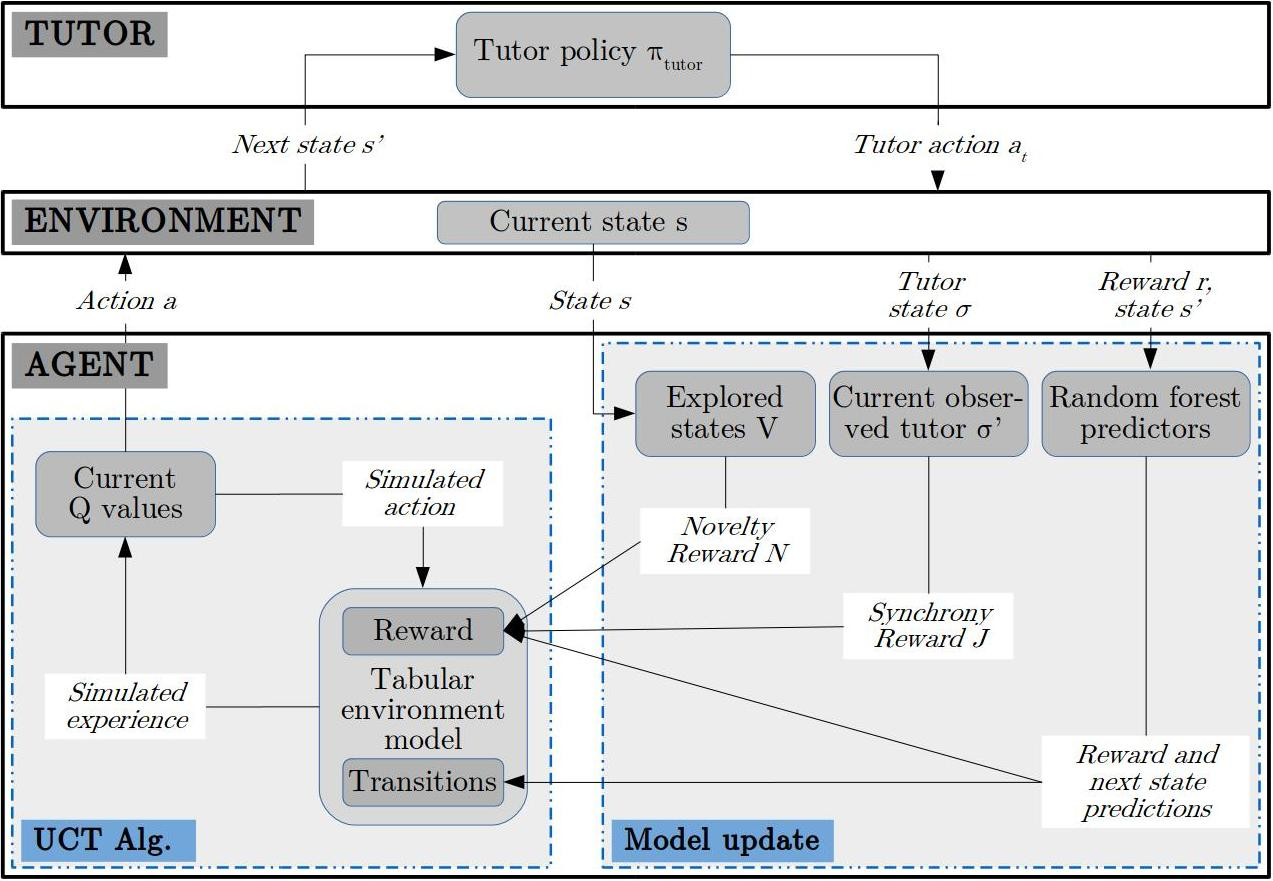
\includegraphics[width=\textwidth]{model.jpg}
  \end{minipage}}
\usebox{0}\hfill
\begin{minipage}[b][\ht0][s]{.3\textwidth}
\vfill
\begin{comment}
\centering
\noindentwriting
\par\footnotesize\begin{tabularx}{\textwidth}{|c|X|}
\hline
\textbf{Task name} & \textbf{Reward $R=100$ for: }\\
\hline
ALL & Any block in any box\\
\hline
MATCHING & Red blocks in red box \& blue blocks in blue box\\
\hline
OPPOSITE & Red blocks in blue box \& blue blocks in red box\\
\hline
RED & Red blocks in red box \\
\hline
\end{tabularx}
\end{comment}
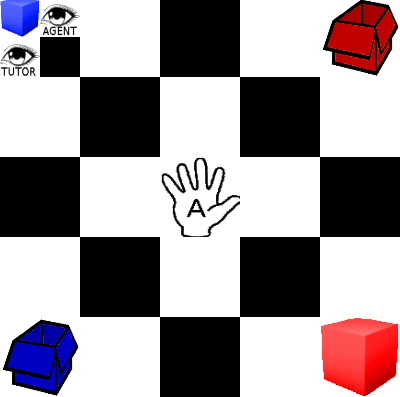
\includegraphics[width=\textwidth]{grid.png}
\end{minipage}
%\captionsetup{forma\mu =hang}
\caption{\textbf{Left}: the agent model is an extension of the classical model-based reinforcement learning scheme, where the tutor behavior is explicitly taken into account to build experience. The agent exploits the accumulated experience to train predictors, from which the tabular environment model is built. Novelty and gaze-based motivations modulate the tabular reward model to favor specific state-action pairs. The agent obtains the best action by computing Q values from simulations based on the environment model. \textbf{Right}: The environment is a 5x5 grid with two sources of red and blue blocks (the cubes) and a box of each color. The agent is defined by its position (the hand) and its actions need to be coordinated with its gaze (its eye). The tutor only exists through its gaze, and he looks where it is best for the agent to also look at. 
%\textbf{Upper right}: tasks and subtasks to be performed by the agent; all consist in picking blocks in order to put them in boxes thereafter. The table shows the task variations with blocks and box colors.
}
\label{model}
\end{figure*}

We augment the \textsc{texplore-vanir} algorithm in two ways: 1) the agent's action achievements are now conditioned to their coordination with its gaze, and 2) a second reward shaping mechanism is added, in order to favor states in which the agent gaze follows the tutor's. 

\subsection{Gaze following motivation}

To fulfill the action-attention coordination constraint, we augment the agent state $s$ with gaze information so that we have now $s=(s^{env},s^{gaze})$ where $s^{env}$ is comprised of pure environment observations from the agent while $s^{gaze}$ is its gaze position. The list of possible actions for the agent in state  $s=(s^{env},s^{gaze})$ is now conditioned to $s^{gaze}$. The next section provides details on these conditions for our specific experimental framework. 

To induce gaze-following behaviors, a new reward $J$ is created based on these gaze-related features: for a given state $s=(s^{env},s^{gaze})$, and a given observation by the agent of the current tutor gaze $\sigma^{obs}$, we write: 
\begin{equation}
\label{eq:j}
J(s,\sigma^{obs}) = \mu \cdot \delta(s^{gaze},\sigma^{obs})
\end{equation} 
where $\delta$ is the Kronecker symbol and $\mu$ a tunable parameter that determines the importance granted to gaze-following behaviors. In short, this reward motivates the agent to choose states where its gaze matches the tutor's. 

\subsection{Algorithm}

The final algorithm structure is shown in Alg.~\ref{algo}, with additional steps relatively to \textsc{texplore-vanir} highlighted. Lines 7-12 comprise building experience that includes the tutor's reactions and training the feature predictors from this experience. Lines 13-17 perform the tabular models updates from the predictors. The reward computations thus include incentives for novelty and gaze-following behaviors by shaping $R$ in \eqref{eq:qupdate} with \eqref{eq:novelty} and \eqref{eq:j}, writing:
\begin{equation}
\label{eq:reward}
\begin{split}
R(s_{t'+k-1},a_{t'+k-1}) & = r_{pred}(s_{t'+k-1},a_{t'+k-1}) \\
& + N(s_{t'+k-1},a_{t'+k-1},V) \\
& + J(s_{t'+k-1},\sigma^{obs}_t).
\end{split}
\end{equation}
It is important to note that $R(s_{t'},a_{t'})$ relies on $\sigma^{obs}_t$ for all $t'$ considered in \eqref{eq:qupdate}: the tutor gaze is not part of the agent state and thus no prediction is made about its future. Thus updates at simulated step $t'$ use the value $\sigma^{obs}$ at step $t$.

Finally line 18 corresponds to the \textsc{uct-planning} algorithm where the Q-table is updated following \eqref{eq:qupdate} and \eqref{eq:reward}. Figure~\ref{model} (left) shows the full model-based learning framework with explicit use of the tutor's gaze signals to modulate the tabular reward model.

\subsection{Experiments}

The algorithm is evaluated on a virtual pick-and-place task in a 5x5 grid world environment, shown in Fig. \ref{model}, right. Two infinite sources of blocks are located in two corners of the grid, while two boxes are located in the remaining corners. The agent must go to a block, pick it up, carry it to a box and place it inside. The agent (the hand in Fig.~\ref{model}) is positioned at the center of the grid at the start of an experiment. The agent must repeatedly put blocks in a box. The positions of the blocks and boxes do not change over time or over trials. The agent state consists of 13 different features: its $x_a$ and $y_a$ coordinates in the room, whether it carries a block, the $x_g$ and $y_g$ coordinates of its gaze, and the $x_i$ and $y_i$ coordinates of all four objects in the grid.

Ten actions are available: the agent can move one step in each cardinal direction, look at all four objects, pick a block and put one in a box. Apart from looking at an object which is always possible, an action realization is conditioned to the environment and to the agent gaze. A move cannot be made against a wall, and the move must be in the direction of the agent gaze (the X coordinate of the gaze must be greater than the X coordinate of the agent to move right for example). To be successful, the pick action (resp. put action) requires the agent to be located at a block position (resp. a box position), while holding nothing (resp. holding a block); its gaze must be directed towards the block (resp. the box). All actions are deterministic and when one is not successful, the agent state remains unchanged.

The tutor's policy in this environment is fixed. Each time the agent ends up holding nothing during exploration, the tutor picks a source of blocks, choosing randomly. Then the tutor keeps looking at the source until the agent takes a block from it. When the agent picks a block, irrespective if it is the one the tutor looked at, the tutor chooses a box at random and looks at it until the agent has placed the block in it. 

%The domains is well-suited to evaluate the contribution of joint attention based motivation as it involves actions that are conditioned to the gaze of the agent in a natural way. Also there is progression of the complexity in the actions: putting a block in a box is harder than picking it up as it requires to already hold one for example. Finally the task itself is convenient for the evaluation of the agent performance on non-stationary reward problems as it is open to several variations with the colors of boxes. 

All experiments consists of 30 trials starting in the exact same conditions (parameters, starting position, etc.). Each trial comprises 800 learning steps, unless otherwise stated. In addition to the accumulated reward, we store for each action $a$ taken in state $s$ the proportions of each of the three rewards in $Q(s,a)$. The parameters $\lambda$, $\gamma$ and $M$ are those of \textsc{texplore-vanir} and remain constant in all experiments: $\lambda = 0.1$, $\gamma = 0.9$ and $M=100$.

\section{Results}
\label{results}

The present model was first designed to measure the impact of the relation between the weight of the incentive for gaze-following and that of curiosity on task discovery in a new environment. In a second phase we evaluate our full motivation system in a reward free version of the environment.

\subsection{Task-oriented exploration}

\begin{figure}[t!]
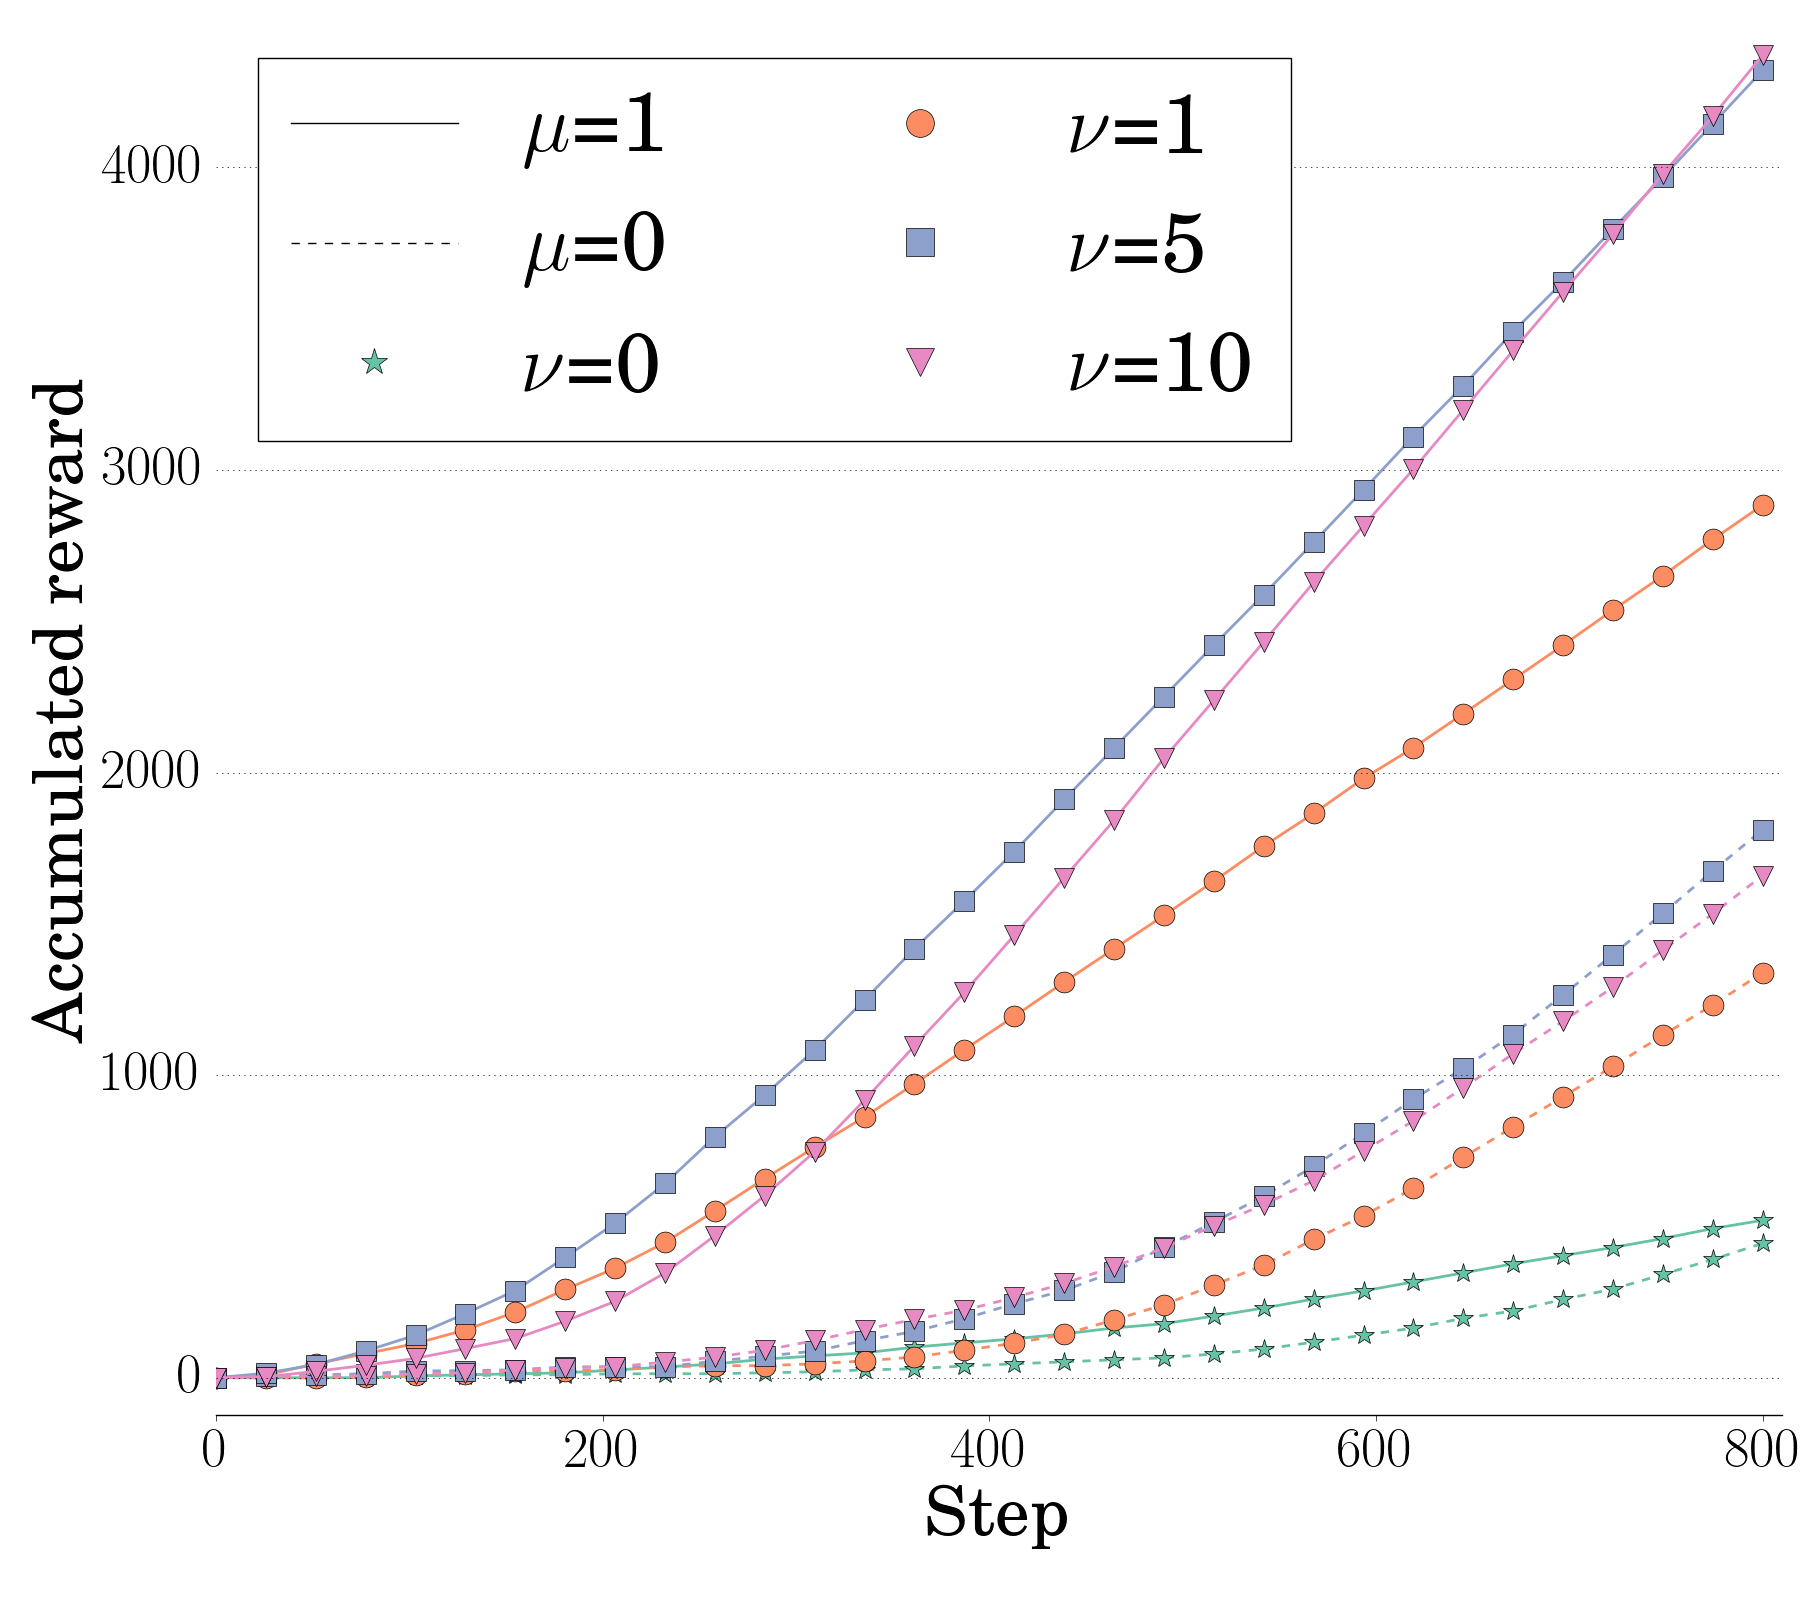
\includegraphics[width=\linewidth]{comparaisonNormale2.png}
\caption{Accumulated reward versus number of steps taken, averaged over 30 trials, with and without a tutor for different parameters n. The incentive to follow the gaze of the tutor clearly facilitates task discovery during the first iterations.}
\label{comparaisonNormale}
\end{figure}

First, the contribution of the tutor during reinforcement learning is examined. Performances of the agent on the pick-and-place task with and without taking the tutor's gaze into account ($\mu =1$ and $\mu =0$) are compared. As we are mainly interested in guiding exploration, we focus on the first few hundreds iterations. Fig. \ref{comparaisonNormale} plots the accumulated rewards versus the number of steps taken by the agent, averaged over 30 trials. The figure shows results for different intrinsic motivation weights: $\mu=0$ and $\mu=1$ on one side, $\nu=0$, $\nu=1$, $\nu=5$ and $\nu=10$ on the other. Experiments where the agent takes the tutor gaze into account appear more efficient at discovering the task than their counterparts with intrinsic motivation only. During the very first iterations, intermediate intrinsic motivation ($\nu=5$) provides the fastest increase in accumulated rewards. However, more curiosity ($\nu=10$) leads to discovering better strategies after a few hundred additional iterations and leads to a better average score at step 800. 

Figure~\ref{comparaisonNormale} shows different performance gains for a constant appeal to joint attention ($\mu=1$) depending on the importance granted to curiosity through $\nu$. This suggests a coupling between intrinsic motivation and gaze-following, which we analyze in Fig. \ref{TB1}. To this end, we make $\nu$ vary between $0$ and $20$ with a fixed $\mu=1$ and focus on the end reward accumulated at step 800 only. For each value of $\nu$, Fig. \ref{TB1} shows on a vertical line the distribution of results obtained over the 30 trials. To account for trials giving identical results, these 30 values are binned in intervals $[0,1000]$, $[1000,2000]$, ..., $[5000,6000]$ and each bin is shown as a circle centered at the average value of the bin, and of size proportionate to the number of elements in the bin. For instance, with no curiosity at all ($\nu=0$, on the left), most trials have not discovered the task nor obtained any reward, hence the large dot on the no-reward horizontal axis, while the task has been discovered by chance in a few trials.

\begin{figure}[t!]
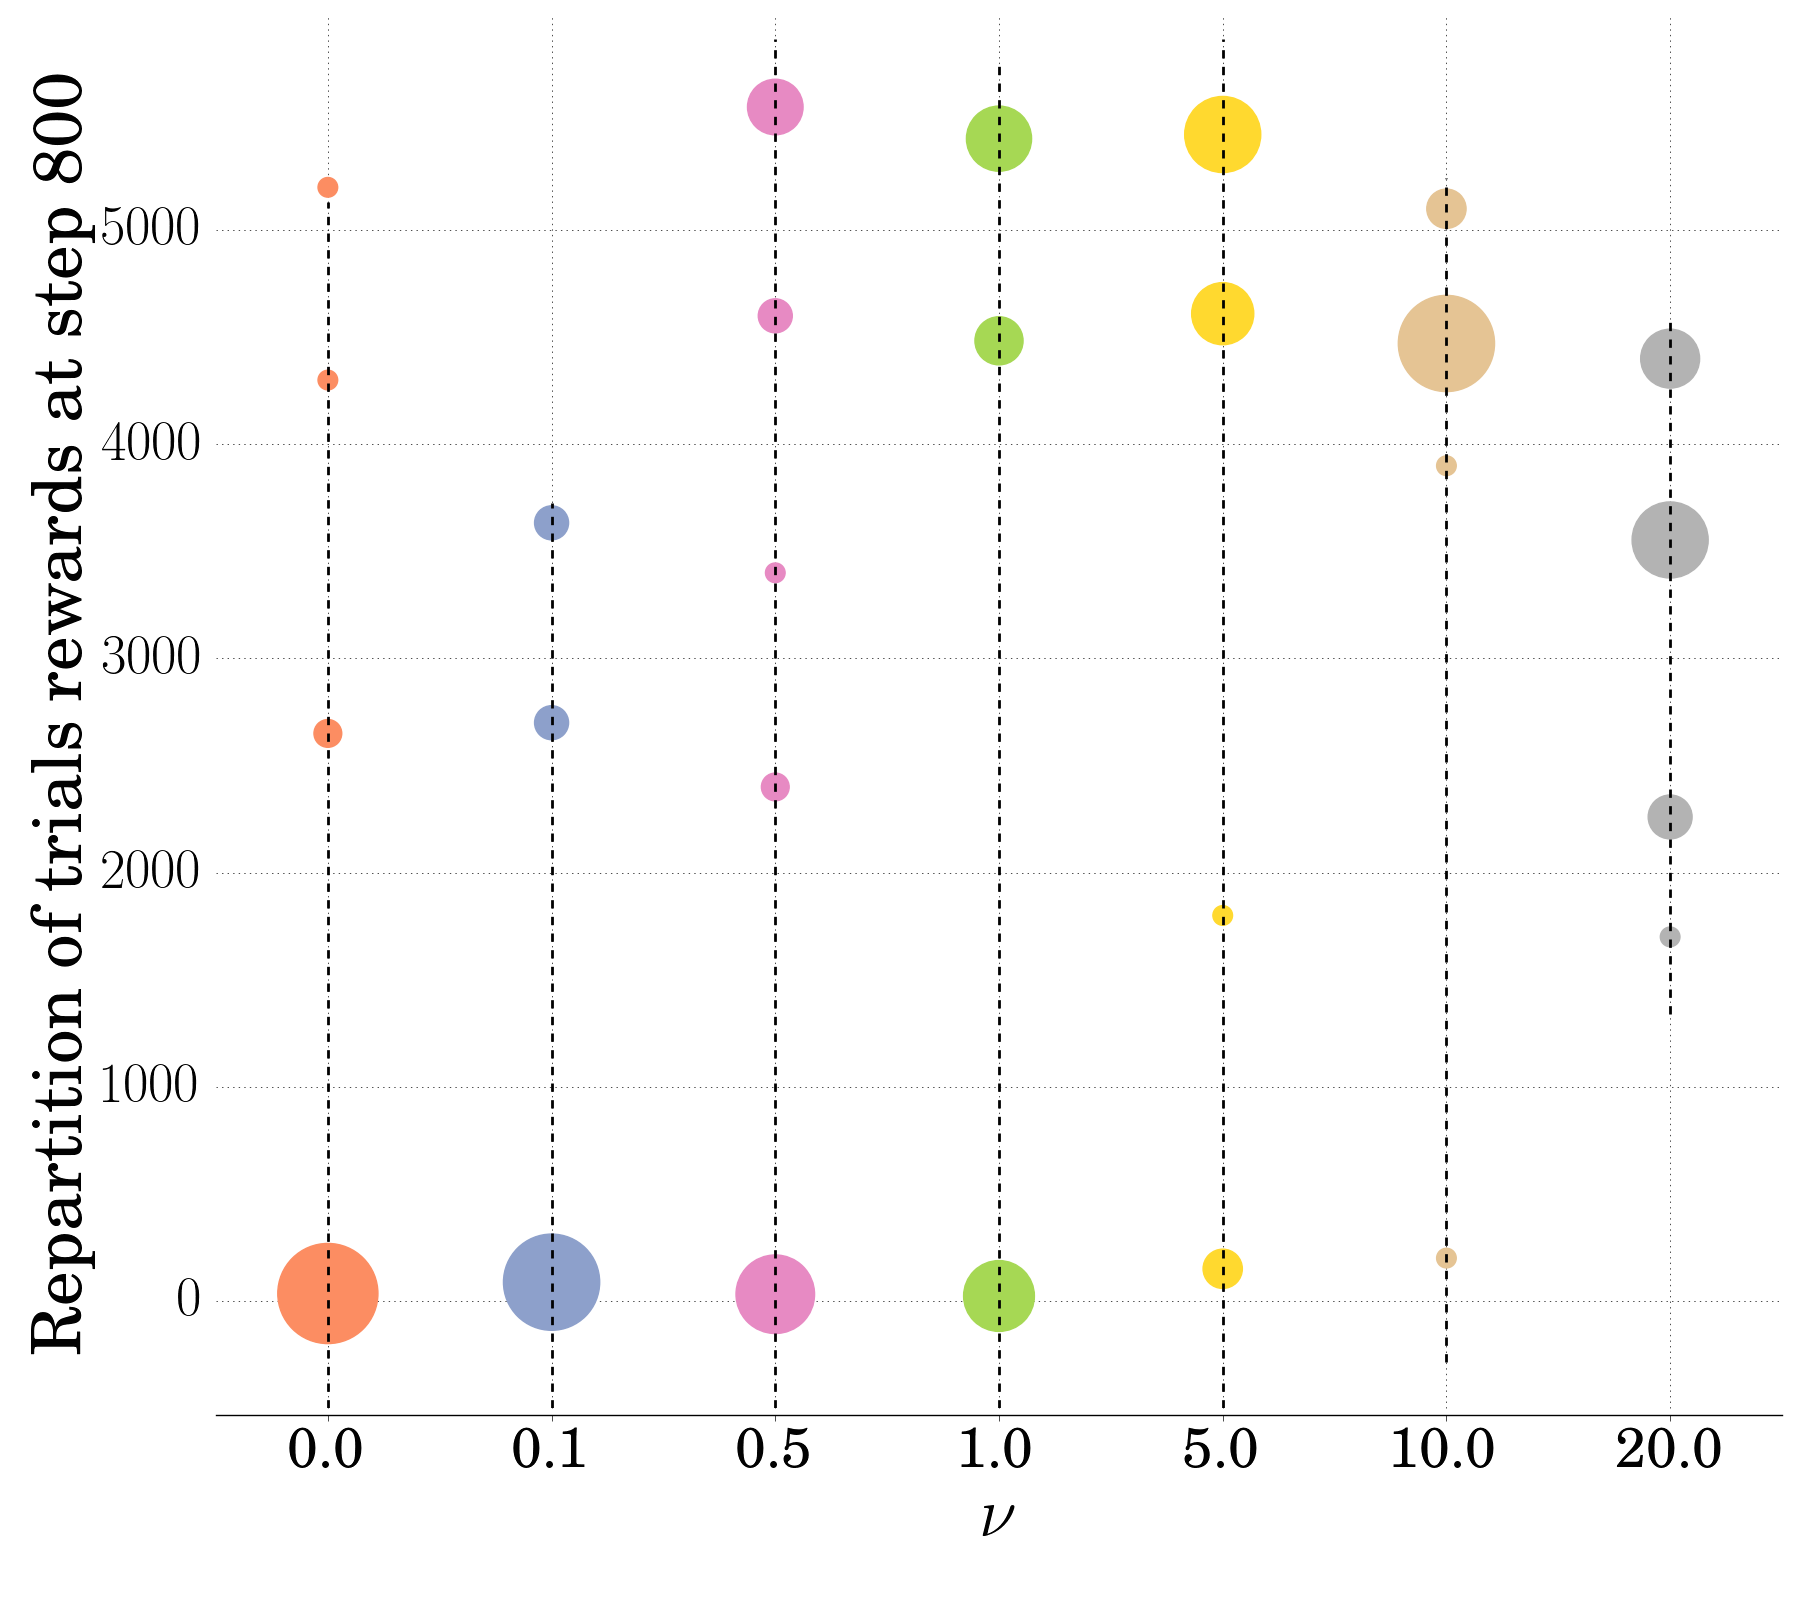
\includegraphics[width=\linewidth]{boxplotstb1.png}
\caption{Distributions of the accumulated reward at step 800 over the 30 trials for different values of $\nu$, each corresponding to a vertical line, for a fixed $\mu=1$. On each vertical, the 30 trial results are binned in the six $[0,1000]$, $[1000,2000]$, ..., $[5000,6000]$ intervals. Each bin is then displayed as a circle at height equal to the average value of the bin and of size proportionate to the number of results in the bin. The best result in term of both accumulated reward and consistency over trials is obtained for $\nu=10$: few low reward results and many high reward results.}
\label{TB1}
\end{figure}

A significant proportion of the trials for $\nu\leq10$ still obtain few to no reward at all, as illustrated by a remaining circle close to zero; on the other hand, the majority of other trials reach high end results as shown by large dots for high intervals. Between these two behaviors lie very few samples. These results indicate that either the agent discovers the task early enough and then exploits its discovery to reach a high final accumulated reward, or it remains stuck in a form of inefficient exploration and receives no reward at all. The absence of intermediate end-result (few values between $1000$ and $4000$ for $0.5 \leq\nu\leq 10$ in particular) is a consequence of this alternative. If we evaluate the chosen parameters based on consistency over trials and on the actual 800 step accumulated reward, performances are best for $\nu=10$ and $\mu=1$.

%Therefore the statistics with the Mann-Whitney U-test on the experiments of Fig.~\ref{comparaisonNormale}, giving the comparisons at $\nu=5$ and $\nu=10$ as highly significant ($p<0.0001$) while not significant at 5\% for $\nu=1$, should be taken with caution. 

%Box plots show the interquartile range ($IQR=Q3-Q1$) while whiskers extend to data between $Q1-1.5\cdot IQR$ and $Q3+1.5\cdot IQR$. The external reward and the task remain identical. When importance granted to novelty is low ($n<0.5$), the agent finds a rewarding course of actions only very rarely as shown by the few high score outliers. On the contrary, for values of $n$ ranging from 5 to 10, high scores at step 800 are the norm, with a narrow $IQR$, while a few low to no reward trials remain as outliers. Between these first ranges of values (for $\nu=0.5$ and $\nu=1$), the agent operates a behavior transition with success and failure trials in closer proportions and a very wide $IQR$. A second behavior transition appears when novelty-based curiosity is given too much credit: performance start to drop when $\nu \geq 20$, with poor trials coexisting with successful ones in increasing proportions.

The observed behavior is easily interpreted in the light of the role played by each reward mechanism during exploration. To measure these roles, we use the proportions of each reward/motivation mechanism inside the Q-value corresponding to the chosen action at each iteration, which we store all along the trials. They indicate how much each reward/motivation mechanism is responsible for the action of the agent. The evolution of these proportions,  shown in Fig.~\ref{fig:prop} on the left for two very different behaviors (weak versus strong curiosity), indicates that low performances on the left of Fig. \ref{TB1} correspond to the agent only looking where the tutor looks, without searching to discover the environment and with growing but weak interest for the task. The decrease in performance observed for high values of $\nu$ stems from the opposite behavior where the agent's goal is the complete discovery of the environment, independently of the task or the tutor. The benefit of this strategy is that it almost guarantees random task execution and avoids no-reward trials. A successful trade-off between curiosity, joint attention and external reward exploitation is reached for $\nu=10$ (Fig.~\ref{fig:prop}, right): novelty-based motivation appears critical at the beginning of learning and then gives way to external reward signal discovered, while the tutor acts as a permanent discrete guidance. This combination leads to a more effective task-oriented exploration of the environment than any of the drives taken separately.


\begin{figure}[t!]
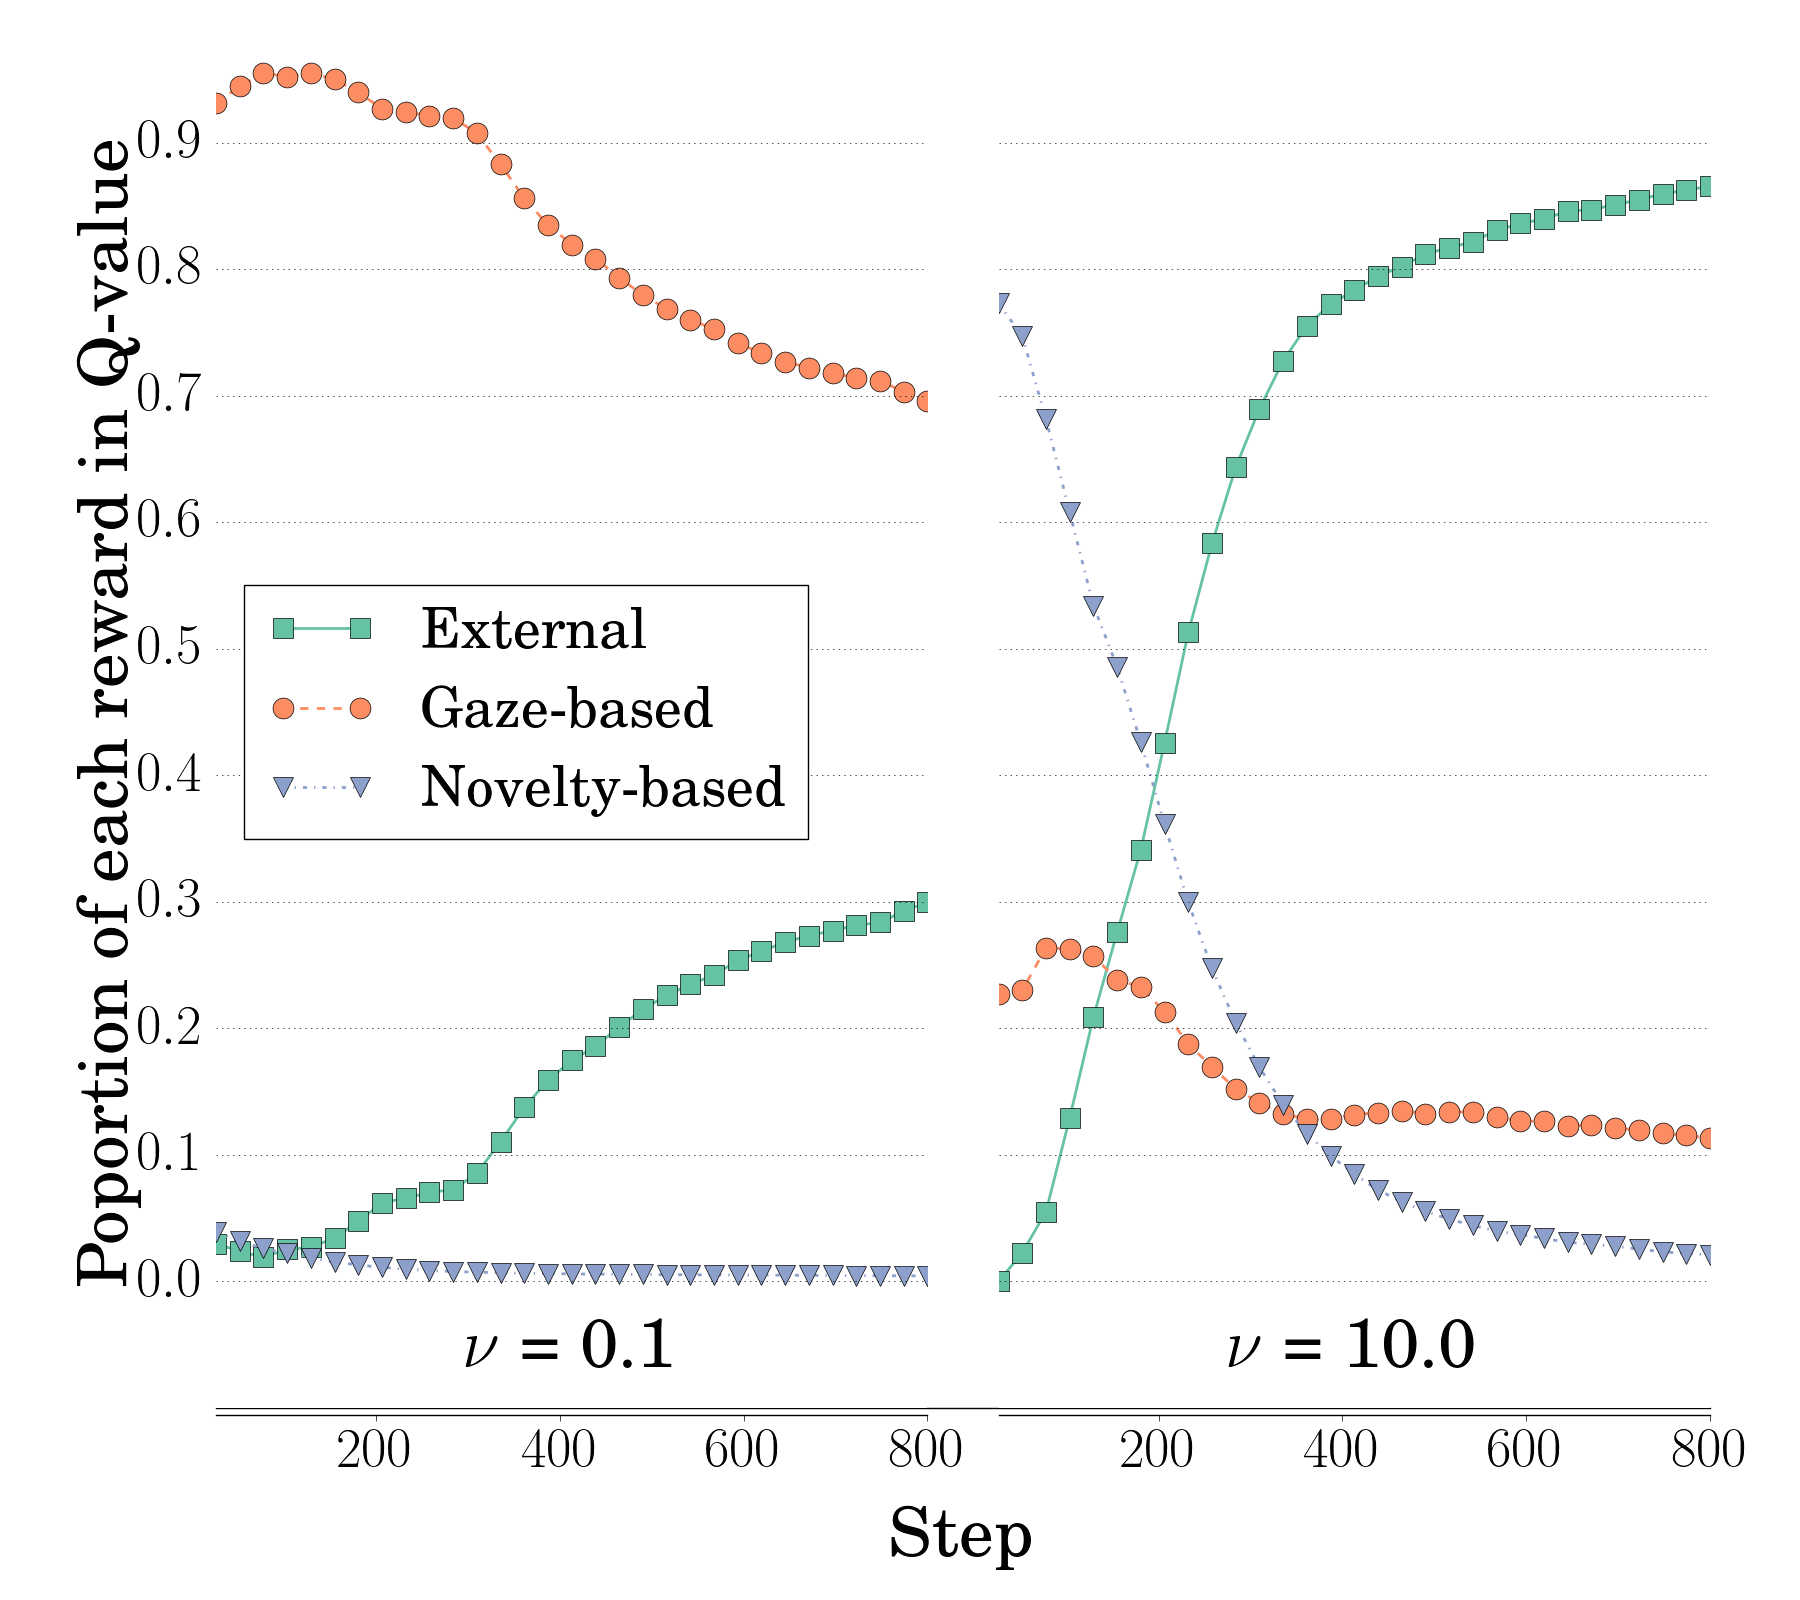
\includegraphics[width=\linewidth]{prop.png}
\caption{Importance of each reward mechanism in action-selection during the first 800 steps, for the two combinations $[\mu=1,\nu=0.1]$ (left) and $[\mu=1, \nu=10]$ (right). The evolution of the proportion of each member of \eqref{eq:reward} in the Q-value defining the next action is displayed. Successful combinations of motivations (right) enable novelty to play the main role at the very beginning and give way to environment rewards when they are discovered, while the tutor guidance impacts the agent with a continuous moderate intensity. An insufficient curiosity leads to following the tutor gaze only (left).}
\label{fig:prop}
\end{figure}

 \subsection{Reward-free environments}

Now the reward obtained from the environment is only used for evaluation purposes and learning only relies on the two last terms of \ref{eq:reward}. The agent is only driven by curiosity and the tutor gaze. Fig. \ref{noreward} shows the impact of the attention-based guidance on the accumulated reward corresponding to the amount of blocks put inside boxes over time. With curiosity only, the agent achieves the task by chance on rare occasions over the 800 steps. By contrast, in presence of a tutor, it discovers the task earlier and more importantly, also achieves the task expected by the tutor with regularity. This ability is obtained through the combination of the two reward mechanisms and the attention-action coordination constraint: schematically the agent attention is first driven to the parts of the state space indicated by the tutor; because of the action-attention coordination constraints, the agent itself is then more likely to actually end up in those states the tutor deems useful; finally, once in those potentially rewarding states, the curiosity mechanism ensures that the agent will find the right action, among those it has not tried yet.

The plot also shows that the binary behavior described in the previous section has been reduced. Indeed, the 25-75 interquartile ranges drawn for each experiment over the 30 corresponding trials indicate that there is far less uncertainty in the end-results without external rewards. Also, the coupling between parameters $\nu$ and $\mu$ still exists without reward: $[\nu=5,\mu =1]$ performs significantly better than both $[\nu=10,\mu =1]$ and $[\nu=1,\mu =1]$ as shown by the non-overlapping interquartile ranges. A comparison with Fig.~\ref{comparaisonNormale} shows that learning without external reward logically remains less efficient than with it. This is coherent with the earlier explanation of task successes: with an external reward obtained when the goal is reached, the agent can propagate it backward in its sequence of actions, so that it knows how to act in each state, which is not possible without reward propagation. 

%In addition to being more developmentally sound, no-reward approaches tackle a difficult problem for classical reinforcement learning: changing environment and tasks. Essentially if state-action pairs that used to be rewarding become neutral, while others become rewarding, a standard Q-learning algorithm will need some time to forget its learned policy and start exploring again. Fig. \ref{changing} evaluates the no-reward system tested before ($R=0$, $\nu>0$ and $\mu>0$) against its counterpart with external reward ($R=100$). For this experiment, trials consisted in a training phase on the task MATCHING (see Fig.~\ref{model}, upper left) for 800 iterations. At step 800, the task becomes OPPOSITE and the numbers of blocks placed in boxes of matching and opposite color are monitored. Fig. \ref{changing} plots the evolution of the proportion of blocks put in the correct box, for various groups of parameters.

\begin{figure}[t!]
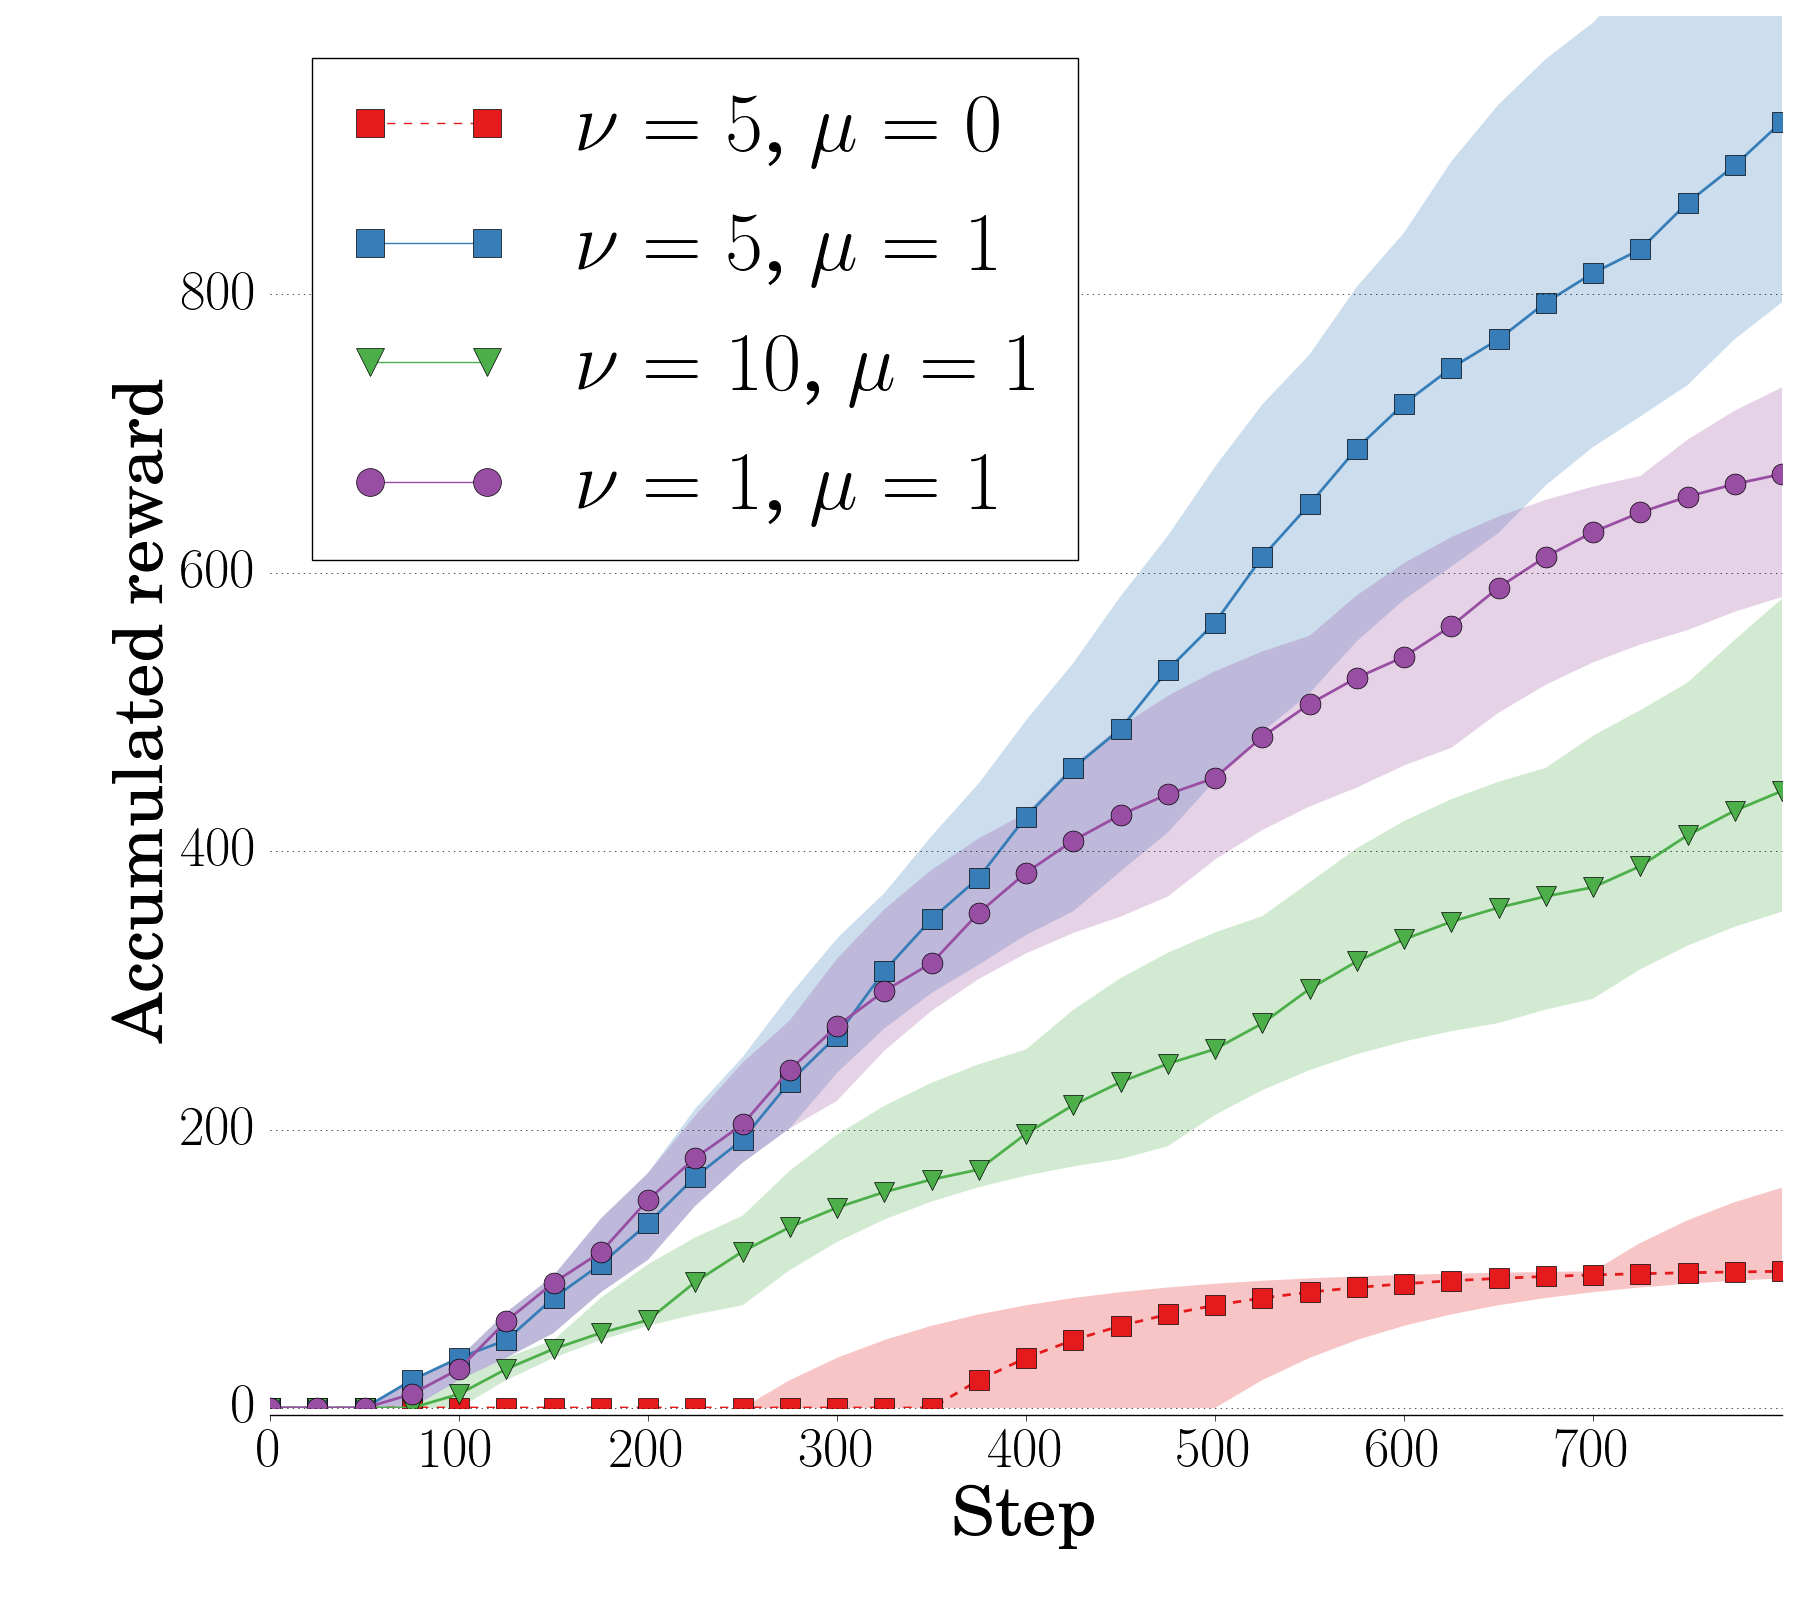
\includegraphics[width=\linewidth]{no_reward.png}
\caption{Evolution of the reward accumulated for putting blocks in boxes over 800 steps (median and 25-75 interquartile range), for different combinations of gaze-based and curiosity-based motivations. Proper combinations of curiosity and interaction drives lead to the task being achieved regularly without using dedicated external rewards.}
\label{noreward}
\end{figure}

%Experiments without external reward (during training as well as after the inversion) exhibit greater reactivity to the task change. Also higher values of parameter $\nu$ (independently of the reward value) facilitate adaptation, as expected. It is worth noticing that the combination of joint attention, intrinsic motivation and external reward remains quite flexible as only a thousand iterations seem necessary for $[R=100, \nu=10, \mu =1]$ to perform the task OPPOSITE more often than MATCHING. In all cases, the increase in reactivity comes from the joint attention naturally taking the agent to parts of the environment where many state-action pairs are motivating, thus triggering the intrinsic motivation system.

\begin{comment}
\begin{figure}[t!]
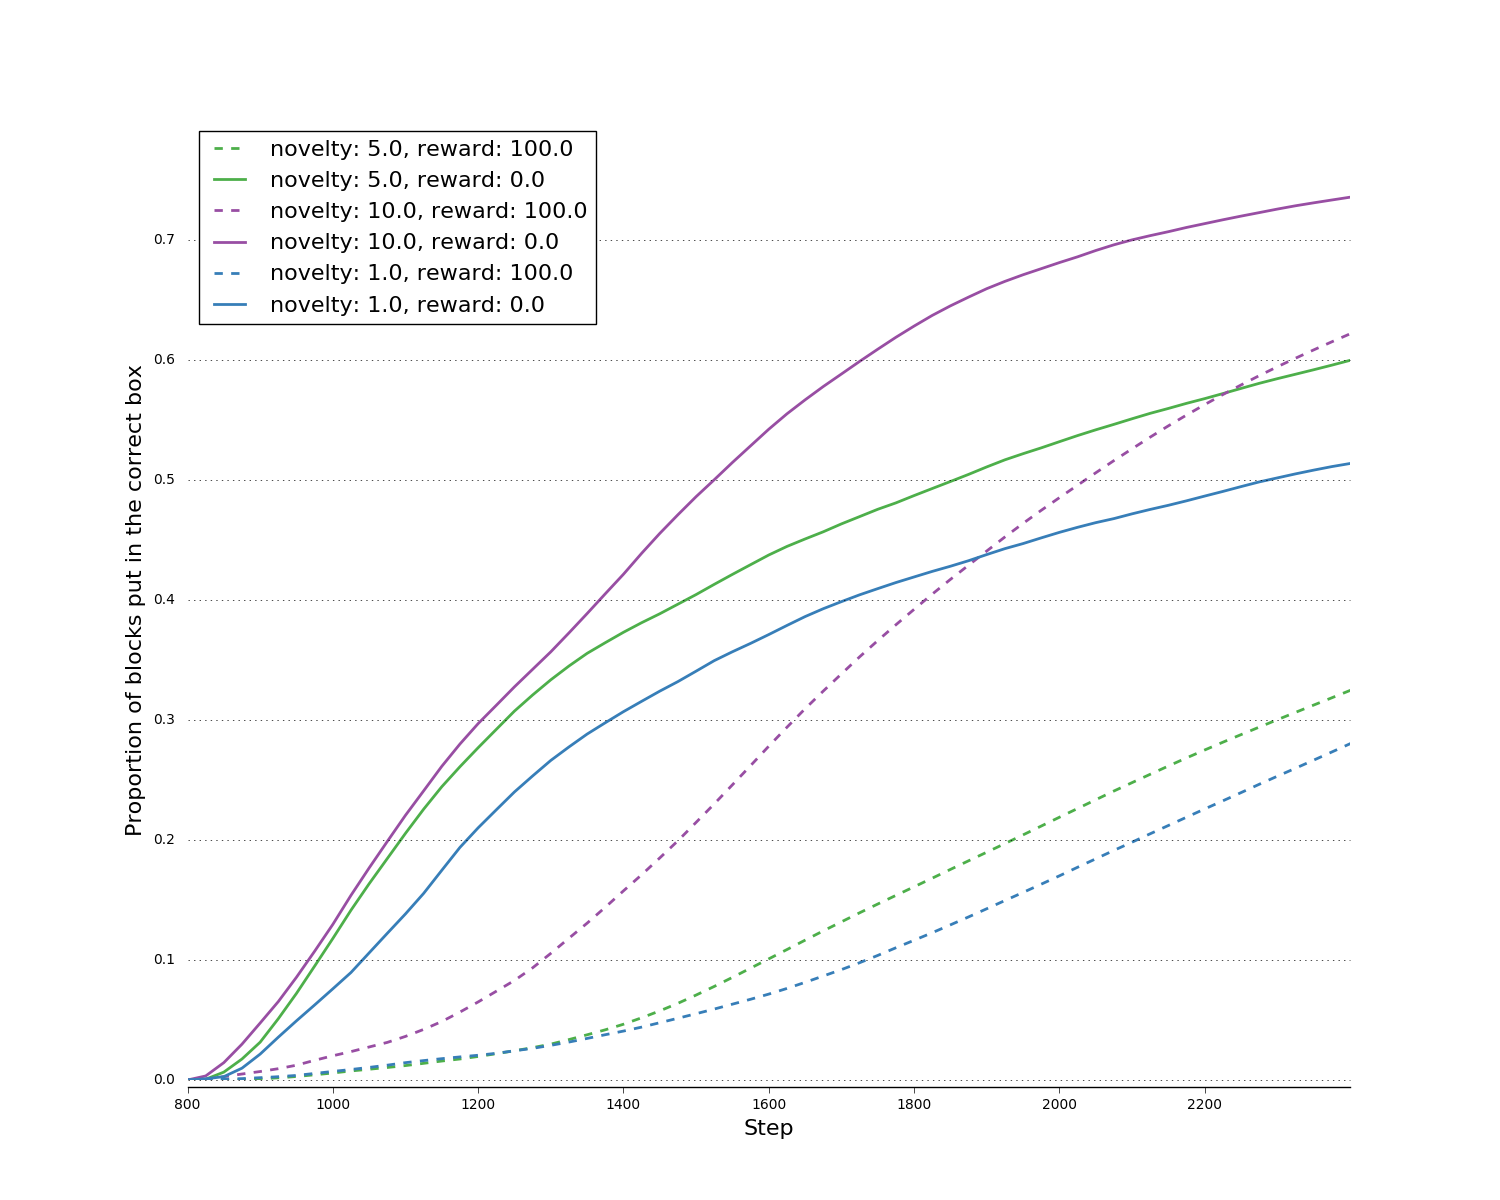
\includegraphics[width=\linewidth]{Flexibility.png}
\caption{Evolution of the proportion of blocks placed inside the right box after task inversion (blocks in boxes of matching versus opposite color) at step 800, in presence of a tutor. Trials without external reward from the environment show more reactivity to the goal change.}
\label{changing}
\end{figure}
\end{comment}

\addtolength{\textheight}{-0cm}   % This command serves to balance the column lengths
                                  % on the last page of the document manually. It shortens
                                  % the textheight of the last page by a suitable amount.
                                  % This command does not take effect until the next page
                                  % so it should come on the page before the last. Make
                                  % sure that you do not shorten the textheight too much.


\section{Conclusion}
\label{conclusion}

In this paper, we presented a generic extension of the RL framework to combine autonomous exploration out of curiosity, and guidance from a tutor based on gaze-following. Contrary to a number of works in IML, such as RL with on line human-defined rewards \cite{knox_interactively_2009}, our solution does not consider interaction as a secondary tool to fulfill a primary objective. Instead, interaction is seen as a goal in itself, and is favored by a dedicated reward mechanism. Also, interaction takes a bottom-up approach and relies on a low-level gaze-based social cue as in other works \cite{broz_learning_2009}. Previous studies following this line of thought have faced difficulties in interpreting such social cues, as it adds complexity to the problem \cite{najar_social-task_2015,lopes_simultaneous_2011,grizou_robot_2013}. Our solution tackles the issue by converting gaze direction into an exploitable guidance through reward shaping in the RL framework. 

Results show that adding a tutor gaze direction as a guidance to a curious RL agent leads to improved exploratory abilities, provided that curiosity and motivation for gaze-following are combined in correct proportions. When such a successful balance is reached, the tutor guidance acts as a constant and moderate push towards profitable states, while curiosity appears decisive at the very beginning of exploration, and fades as it goes on. With this behavior, the agent performs better at task-discovery and execution than other combinations of curiosity and guidance by tutoring signals, or without guidance at all.  

\emph{Results show a strong dependency of the agent performances on the relation between curiosity and the motivation for gaze-following. With a successful balance, the tutor guidance acts as a constant and moderate push towards profitable states, while curiosity appears decisive at the very beginning of exploration, and fades as exploration goes on. When such behaviors are obtained, the agent performs better at task-discovery and execution than any other combination of both motivations, or without guidance from a tutor.} 

As the few studies that have tackled the issue of autonomous reward-free environment discovery, our curiosity mechanism mainly relies on the agent evaluating its internal model of the environment \cite{oudeyer_playground_2005,little_learning_2013}. This evaluation then serves as a basis for directing exploratory behavior. Our work demonstrates that the exploitation of a guidance signal in tuned proportion is also an effective solution to speed up task discovery and regular execution in such reward-free environments.

Future work should further elaborate the gaze following mechanism which is hitherto oversimplified: the tutor gaze direction is given whereas it should be detected. This causes the agent to follow its tutor too easily instead of learning gaze following \cite{carlson_computational_2004}. Results can also be improved by automatic goal-discovery \cite{forestier_autonomous_2016} and tutor intentions inference \cite{diaconescu_inferring_2014}. Both would enable subgoal-based rewards and competence-based motivations \cite{forestier_towards_2015} that would speed up exploration and make guidance more efficient.


%%%%%%%%%%%%%%%%%%%%%%%%%%%%%%%%%%%%%%%%%%%%%%%%%%%%%%%%%%%%%%%%%%%%%%%%%%%%%%%%


%%%%%%%%%%%%%%%%%%%%%%%%%%%%%%%%%%%%%%%%%%%%%%%%%%%%%%%%%%%%%%%%%%%%%%%%%%%%%%%%



%%%%%%%%%%%%%%%%%%%%%%%%%%%%%%%%%%%%%%%%%%%%%%%%%%%%%%%%%%%%%%%%%%%%%%%%%%%%%%%%

\begin{comment}
\section*{APPENDIX}

Appendixes should appear before the acknowledgment.

\section*{ACKNOWLEDGMENT}

The preferred spelling of the word ÒacknowledgmentÓ in America is without an ÒeÓ after the ÒgÓ. Avoid the stilted expression, ÒOne of us (R. B. G.) thanks . . .Ó  Instead, try ÒR. B. G. thanksÓ. Put sponsor acknowledgments in the unnumbered footnote on the first page.

\end{comment}

\bibliographystyle{ieeetr}
\bibliography{Zotero.bib}

\end{document}
